\documentclass[
  11pt,
  letterpaper,
   addpoints,
   answers
  ]{exam}

% Carga el preámbulo localizado en la carpeta superior
\input{../exercise-preamble.sty}
% Paquetes locales
\usepackage{float}
\usepackage{booktabs} % para \toprule, \midrule, \bottomrule
\usepackage{xcolor} % para colores
\usepackage{bm} % para negrita en símbolos matemáticos
\usepackage{empheq} % para ecuaciones enmarcadas

% Macros locales
\newcommand{\Rel}{\mathfrak{R}} % símbolo para la reluctancia
\DeclareMathOperator{\Var}{Var} % operador de varianza

\begin{document}

% Configuración del encabezado usando comandos de la clase exam
\pagestyle{headandfoot}
\extraheadheight{0.5in} % Baja el encabezado aumentando el espacio superior
\firstpageheader{\textit{Análisis de Sistemas Dinámicos y Estimación}}{}{EL3204-1}
\runningheader{\textit{Análisis de Sistemas Dinámicos y Estimación}}{}{EL3204}
\firstpagefooter{}{\thepage}{}
\runningfooter{}{\thepage}{}
\headrule % Línea debajo del encabezado

% Numeración de página
\pagenumbering{arabic}

% Portada
\begin{center}
    \vspace*{1cm}
    
    % Logo superior
    
\includegraphics[width=0.5\textwidth]{../fcfm_die}
    
    \vspace{2cm}
    
    % Líneas decorativas superiores
    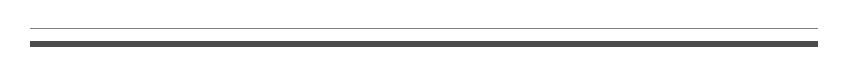
\begin{tikzpicture}
        \draw[line width=2pt, black!70] (0,0) -- (10,0);
        \draw[line width=0.5pt, black!50] (0,0.2) -- (10,0.2);
    \end{tikzpicture}
    
    \vspace{1cm}
    
    % Título principal
    {\fontsize{28}{34}\selectfont\bfseries 
    Análisis de Sistemas\\[0.3cm]
    Dinámicos y Estimación}
    
    \vspace{0.5cm}
    
    {\Large\textbf{EL3204-1}}
    
    \vspace{1cm}
    
    % Líneas decorativas inferiores
    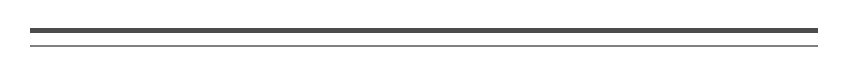
\begin{tikzpicture}
        \draw[line width=0.5pt, black!50] (0,0) -- (10,0);
        \draw[line width=2pt, black!70] (0,0.2) -- (10,0.2);
    \end{tikzpicture}
    
    \vspace{1.5cm}
    
    % Subtítulo
    {\LARGE\itshape Pauta Auxiliar 13 - Repaso Examen}
    
    \vspace{0.5cm}
    {\large Prof Marcos Orchard - Sebastian Espinoza.}\\
    {\large Prof Auxiliar Erik Sáez Aravena.}
    
    % Decoración con símbolo matemático de fondo
    \begin{tikzpicture}[remember picture, overlay]
        \node[opacity=0.5, rotate=0] at ([yshift=-8cm]current page.center) {
            \fontsize{280}{300}\selectfont\color{black!15}$\mathcal{I}(\theta)$
        };
    \end{tikzpicture}
    
    \vfill
    
\end{center}

\newpage
%----------------------------
% =========================================
% Unidad III — Estimación de Parámetros (Resumen)
% =========================================
\section*{Resumen}

Este auxiliar cubre conceptos fundamentales de la teoría de estimación de parámetros, que complementa los temas de detección vistos anteriormente. En problemas de detección, el espacio paramétrico $\Theta$ era discreto y finito, pero ahora trabajamos con un conjunto \textbf{infinito no numerable} de posibles valores para el parámetro que queremos estimar (un continuo).

\subsection*{1. Conceptos Básicos de Estimación}
Algunos conceptos importante a considerar son:
\begin{enumerate}
\item \textbf{Espacio de observación ($\mathbb{X}$):} Espacio donde la variable aleatoria $X \in \mathbb{X}$ toma valores. Para vectores aleatorios, $\mathbb{X}^n$ representa el espacio producto.

  \item  \textbf{Espacio de decisión ($\Theta$):} En estimación, es un conjunto \textbf{infinito no numerable} de valores (a diferencia de detección donde era finito). Ejemplos: $\Theta = \mathbb{R}^+$ para estimar amplitudes, $\Theta = \mathbb{R}$ para estimar medias.

\item \textbf{Familia de distribuciones paramétricas ($J_\theta$):} Conjunto de distribuciones indexadas por $\theta$:
\[
J_\theta = \{P_X(x|\theta) : \theta \in \Theta\}
\]

\item \textbf{Estimador:} Una función $\hat{\theta}(x_1, \ldots, x_n)$ que depende de las observaciones y entrega una estimación del parámetro $\theta$ asociado a la distribución $P_X(x|\theta)$.
\end{enumerate}
\subsection*{2. Propiedades de los Estimadores}
\begin{enumerate}
  \item \textbf{Estimador Insesgado:} Un estimador $\hat{\theta}(x_1, \ldots, x_n)$ es insesgado si:
\[
\mathbb{E}[\hat{\theta}(X_1, \ldots, X_n)] = \theta
\]
Es decir, en promedio el estimador entrega el valor verdadero del parámetro.

\item \textbf{Estimador Asintóticamente Insesgado:} Si el sesgo tiende a cero cuando $n \to \infty$:
\[
\lim_{n\to\infty} \mathbb{E}[\hat{\theta}(X_1, \ldots, X_n)] = \theta
\]

\item \textbf{Estimador Consistente:} Un estimador es consistente si converge en probabilidad al valor verdadero:
\[
\lim_{n\to\infty} P_X(|\hat{\theta}(X_1, \ldots, X_n) - \theta| > \epsilon) = 0 \quad \forall \epsilon > 0
\]

\item \textbf{Observación:} Mediante la desigualdad de Chebyshev, si un estimador es insesgado y su varianza tiende a cero cuando $n \to \infty$, entonces es consistente:
\[
\lim_{n\to\infty} \Var(\hat{\theta}(X_1, \ldots, X_n)) = 0 \implies \text{consistencia}
\]
\end{enumerate}
\subsection*{3. Condiciones de Regularidad}

Las condiciones de regularidad permiten intercambiar el orden de derivación e integración en la función de verosimilitud. Bajo estas condiciones se cumple:
\begin{enumerate}
  \item \textbf{Primera condición:} La esperanza de la derivada de la log-verosimilitud es cero:
\[
\mathbb{E}_{X_1^n}\left[\frac{\partial \ln L(X_1, \ldots, X_n|\theta)}{\partial \theta}\right] = 0
\]

\item \textbf{Segunda condición:} La esperanza de un término específico es cero:
\[
\mathbb{E}_{X_1^n}\left[\frac{1}{L(X_1, \ldots, X_n|\theta)}\frac{\partial^2 L(X_1, \ldots, X_n|\theta)}{\partial \theta^2}\right] = 0
\]

\item \textbf{Identidad de Bartlett:} Relaciona la varianza con su segunda derivada:
\[
\mathbb{E}_{X_1^n}\left[\left(\frac{\partial \ln L}{\partial \theta}\right)^2\right] = -\mathbb{E}_{X_1^n}\left[\frac{\partial^2 \ln L}{\partial \theta^2}\right]
\]

Esta identidad permite calcular la información de Fisher de dos formas equivalentes.
\end{enumerate}
\subsection*{4. Información de Fisher}

La información de Fisher $\mathcal{I}(\theta)$ cuantifica cuánta información sobre el parámetro $\theta$ contienen las observaciones:
\[
\mathcal{I}(\theta) = \mathbb{E}\left[\left(\frac{\partial \ln f(X|\theta)}{\partial \theta}\right)^2\right] = -\mathbb{E}\left[\frac{\partial^2 \ln f(X|\theta)}{\partial \theta^2}\right]
\]

\textbf{Propiedad Aditiva:} Para muestras i.i.d., la información de Fisher es aditiva:
\[
\mathcal{I}_n(\theta) = n \cdot \mathcal{I}_1(\theta)
\]

Esta propiedad refleja que más observaciones independientes proporcionan más información sobre el parámetro.

\subsection*{5. Cota de Cramér-Rao}

La cota de Cramér-Rao establece un límite inferior para la varianza de cualquier estimador insesgado:
\[
\Var(\hat{\theta}) \geq \frac{1}{\mathcal{I}(\theta)}
\]
\begin{enumerate}
  \item \textbf{Estimador Eficiente:} Un estimador insesgado que alcanza la cota de Cramér-Rao se llama \textbf{eficiente} o \textbf{de mínima varianza}

\item \textbf{Interpretación:} La información de Fisher es inversamente proporcional a la mínima varianza posible. Más información $\implies$ menor varianza mínima.
\end{enumerate}
\subsection*{6. Estimador de Máxima Verosimilitud (ML)}

El estimador de máxima verosimilitud se obtiene maximizando la función de verosimilitud:
\[
\hat{\theta}_{ML} = \arg\max_{\theta} L(x_1, \ldots, x_n|\theta) = \arg\max_{\theta} \ln L(x_1, \ldots, x_n|\theta)
\]

\textbf{Método de solución:} Criterio de la primera derivada:
\[
\frac{\partial \ln L(x_1, \ldots, x_n|\theta)}{\partial \theta}\bigg|_{\theta=\hat{\theta}_{ML}} = 0
\]

Verificar que la segunda derivada es negativa para confirmar que es un máximo.

\subsection*{7. Estimación Bayesiana}

En el enfoque bayesiano, el parámetro $\theta$ es considerado como una variable aleatoria con una distribución a priori $P_{\Theta}(\theta)$ o $f_{\Theta}(\theta)$. Se busca encontrar estimadores basados en la distribución a posteriori:
\[
f_{\Theta|X}(\theta|x) = \frac{f_{X|\Theta}(x|\theta) f_{\Theta}(\theta)}{f_X(x)}
\]
\begin{itemize}
\item \textbf{Estimador MMSE (Minimum Mean Square Error):}

El estimador que minimiza el error cuadrático medio es la esperanza condicional:
\[
\hat{\theta}_{MMSE}(x) = \mathbb{E}[\Theta|X=x] = \int_{-\infty}^{\infty} \theta \cdot f_{\Theta|X}(\theta|x) d\theta
\]

Para el caso discreto:
\[
\hat{\theta}_{MMSE}(x) = \sum_{\theta} \theta \cdot P_{\Theta|X}(\theta|x)
\]

\item \textbf{Estimador MAP (Maximum A Posteriori):}

El estimador MAP maximiza la distribución a posteriori:
\[
\hat{\theta}_{MAP}(x) = \arg\max_{\theta} f_{\Theta|X}(\theta|x) = \arg\max_{\theta} f_{X|\Theta}(x|\theta) f_{\Theta}(\theta)
\]

Para el caso discreto:
\[
\hat{\theta}_{MAP}(x) = \arg\max_{\theta} P_{\Theta|X}(\theta|x) = \arg\max_{\theta} P_{X|\Theta}(x|\theta) P_{\Theta}(\theta)
\]

En la práctica se trabaja con el logaritmo:
\[
\hat{\theta}_{MAP}(x) = \arg\max_{\theta} \ln f_{X|\Theta}(x|\theta) + \ln f_{\Theta}(\theta)
\]
\end{itemize}

%----------------------------
\newpage
\begin{questions}
\question El caso de distribuciones exponenciales es emblemático tanto por su simplicidad analítica, así como por su uso como modelamiento del tiempo de falla en sistemas complejos. Consideremos $\overline{\mathbb{X}} = \mathbb{R}^n$, $\Theta = \mathbb{R}^+$ y una secuencia $X_1^n = X_1, ..., X_n$ de variables aleatorias independientes e idénticamente distribuidas (i.i.d.) tales que $X_i \sim Exponencial\left(\frac{1}{\lambda}\right)$, $i \in \{1, ..., n\}$ con $\lambda > 0$ un parámetro.

\textit{Indicación:} Si $X \sim Exponencial(a)$ entonces su función de densidad de probabilidad es
\[
f_X(x) = \begin{cases}
ae^{-ax} & \text{para } x > 0 \\
0 & \text{para } x \leq 0
\end{cases}
\]

Donde además $\mathbb{E}(X) = \frac{1}{a}$ y $Var(X) = \frac{1}{a^2}$.

\begin{parts}
\part[1] Obtenga el estimador de máxima verosimilitud $\hat{\lambda}_{ML}(\cdot)$ del parámetro $\lambda$.

\begin{solution}
\subsection*{Resolución (a): Estimador de Máxima Verosimilitud}

Para encontrar el estimador de máxima verosimilitud, primero escribimos la función de verosimilitud. Dado que $X_1, \ldots, X_n$ son i.i.d. con $X_i \sim \text{Exponencial}(1/\lambda)$:

\begin{equation}
L(x_1, \ldots, x_n|\lambda) = \prod_{i=1}^{n} f_{X_i}(x_i|\lambda) = \prod_{i=1}^{n} \frac{1}{\lambda}e^{-x_i/\lambda} = \frac{1}{\lambda^n} e^{-\sum_{i=1}^{n} x_i/\lambda}
\end{equation}

Tomando el logaritmo natural:
\begin{equation}
\ln L(x_1, \ldots, x_n|\lambda) = -n\ln\lambda - \frac{1}{\lambda}\sum_{i=1}^{n} x_i
\end{equation}

Para encontrar el máximo, derivamos con respecto a $\lambda$ e igualamos a cero (condición de primer orden):
\begin{equation}
\frac{\partial \ln L}{\partial \lambda} = -\frac{n}{\lambda} + \frac{1}{\lambda^2}\sum_{i=1}^{n} x_i = 0
\end{equation}

\textbf{¿Por qué igualamos la derivada a cero?} Porque en cálculo diferencial, los puntos críticos de una función (máximos, mínimos o puntos de inflexión) ocurren donde la derivada es cero o no existe. Cuando la derivada es cero, la pendiente de la función es horizontal en ese punto.

Resolviendo para $\lambda$:
\begin{align}
\frac{1}{\lambda^2}\sum_{i=1}^{n} x_i &= \frac{n}{\lambda}\\
\sum_{i=1}^{n} x_i &= n\lambda\\
\lambda &= \frac{1}{n}\sum_{i=1}^{n} x_i = \bar{x}
\end{align}

\textbf{¿Por qué este valor es el máximo?} Encontramos que $\lambda = \bar{x}$ es un \textbf{punto crítico}. Ahora debemos verificar que efectivamente es un \textbf{máximo} (y no un mínimo o punto de inflexión). Para esto, usamos el \textbf{criterio de la segunda derivada}:

Calculamos la segunda derivada de $\ln L$ con respecto a $\lambda$:
\begin{equation}
\frac{\partial^2 \ln L}{\partial \lambda^2} = \frac{\partial}{\partial \lambda}\left(-\frac{n}{\lambda} + \frac{1}{\lambda^2}\sum_{i=1}^{n} x_i\right) = \frac{n}{\lambda^2} - \frac{2}{\lambda^3}\sum_{i=1}^{n} x_i
\end{equation}

Evaluando en el punto crítico $\lambda = \bar{x} = \frac{1}{n}\sum_{i=1}^{n} x_i$:
\begin{equation}
\frac{\partial^2 \ln L}{\partial \lambda^2}\bigg|_{\lambda=\bar{x}} = \frac{n}{\bar{x}^2} - \frac{2}{\bar{x}^3}\sum_{i=1}^{n} x_i = \frac{n}{\bar{x}^2} - \frac{2}{\bar{x}^3}(n\bar{x}) = \frac{n}{\bar{x}^2} - \frac{2n}{\bar{x}^2} = -\frac{n}{\bar{x}^2} < 0
\end{equation}

\textbf{Interpretación del criterio de la segunda derivada:}
\begin{itemize}
\item Si $\frac{\partial^2 \ln L}{\partial \lambda^2} < 0$ (negativa): La función es \textbf{cóncava} en ese punto $\Rightarrow$ \textbf{MÁXIMO}
\item Si $\frac{\partial^2 \ln L}{\partial \lambda^2} > 0$ (positiva): La función es \textbf{convexa} en ese punto $\Rightarrow$ MÍNIMO
\end{itemize}

Como la segunda derivada es \textbf{negativa} para todo $\lambda > 0$, confirmamos que $\lambda = \bar{x}$ es efectivamente un \textbf{máximo}. Además, como la función es cóncava en todo su dominio (segunda derivada siempre negativa), este máximo es \textbf{único y global}.

Por lo tanto, el estimador de máxima verosimilitud es:
\begin{empheq}[box=\fbox]{equation}
\hat{\lambda}_{ML}(x_1, \ldots, x_n) = \frac{1}{n}\sum_{i=1}^{n} x_i = \bar{x}
\end{empheq}
\end{solution}

\part[1] Calcule sesgo y varianza del estimador obtenido en la parte \textbf{(a)}.

\begin{solution}
\subsection*{Resolución (b): Sesgo y Varianza del Estimador ML}

 Calculamos $\mathbb{E}[\hat{\lambda}_{ML}]$:
\begin{align}
\mathbb{E}[\hat{\lambda}_{ML}] &= \mathbb{E}\left[\frac{1}{n}\sum_{i=1}^{n} X_i\right] = \frac{1}{n}\sum_{i=1}^{n} \mathbb{E}[X_i]\\
&= \frac{1}{n}\sum_{i=1}^{n} \lambda = \frac{n\lambda}{n} = \lambda
\end{align}

Por lo tanto, $\hat{\lambda}_{ML}$ es un \textbf{estimador insesgado}.

\textbf{Varianza:} Como las $X_i$ son independientes:
\begin{align}
\Var(\hat{\lambda}_{ML}) &= \Var\left(\frac{1}{n}\sum_{i=1}^{n} X_i\right) = \frac{1}{n^2}\sum_{i=1}^{n} \Var(X_i)\\
&= \frac{1}{n^2}\sum_{i=1}^{n} \lambda^2 = \frac{n\lambda^2}{n^2} = \frac{\lambda^2}{n}
\end{align}

\begin{empheq}[box=\fbox]{equation}
\Var(\hat{\lambda}_{ML}) = \frac{\lambda^2}{n}
\end{empheq}
\end{solution}

\part[1] Demuestre, bajo condiciones de regularidad, que la Información de Fisher admite la siguiente igualdad:
\[
\mathcal{I}_n(\lambda) = \mathbb{E}_{X_1,...,X_n}\left\{\left(\frac{\partial \ln L(X_1, X_2, ..., X_n|\lambda)}{\partial \lambda}\right)^2\right\} = -\mathbb{E}_{X_1,...,X_n}\left\{\frac{\partial^2 \ln L(X_1, X_2, ..., X_n|\lambda)}{\partial \lambda^2}\right\}.
\]

\begin{solution}
\subsection*{Resolución (c): Igualdad de la Información de Fisher}

Para demostrar esta identidad, utilizaremos las siguientes condiciones de regularidad que permiten intercambiar el orden de derivación e integración:

\textbf{Primera condición de regularidad:} La esperanza de la primera derivada de la log-verosimilitud es cero:
\begin{equation}
\mathbb{E}_{X_1^n}\left[\frac{\partial \ln L(X_1, \ldots, X_n|\lambda)}{\partial \lambda}\right] = 0
\end{equation}

\textbf{Segunda condición de regularidad:} La esperanza de un término específico es cero:
\begin{equation}
\mathbb{E}_{X_1^n}\left[\frac{1}{L(X_1, \ldots, X_n|\lambda)}\frac{\partial^2 L(X_1, \ldots, X_n|\lambda)}{\partial \lambda^2}\right] = 0
\end{equation}

Partimos de la primera condición de regularidad:
\[
\mathbb{E}_{X_1^n}\left[\frac{\partial \ln L(X_1, \ldots, X_n|\lambda)}{\partial \lambda}\right] = 0
\]

Y derivamos ambos lados de esta ecuación respecto a $\lambda$. Del lado izquierdo, bajo condiciones de regularidad podemos intercambiar la derivada con la esperanza (que es una integral):
\[
\frac{\partial}{\partial \lambda}\underbrace{\mathbb{E}_{X_1^n}\left[\frac{\partial \ln L(X_1, \ldots, X_n|\lambda)}{\partial \lambda}\right]}_{= 0} = \mathbb{E}_{X_1^n}\left[\frac{\partial^2 \ln L(X_1, \ldots, X_n|\lambda)}{\partial \lambda^2}\right]
\]

Del lado derecho, derivamos la constante $0$:
\[
\frac{\partial}{\partial \lambda}(0) = 0
\]

Por lo tanto:
\[
\mathbb{E}_{X_1^n}\left[\frac{\partial^2 \ln L(X_1, \ldots, X_n|\lambda)}{\partial \lambda^2}\right] = 0
\]

Este resultado nos dice que la esperanza de la segunda derivada de la log-verosimilitud es cero. Ahora necesitamos conectar estos dos resultados. Partimos de la propiedad fundamental del logaritmo aplicada a la función de verosimilitud:
\[
\frac{\partial \ln L(X_1, \ldots, X_n|\lambda)}{\partial \lambda} = \frac{1}{L(X_1, \ldots, X_n|\lambda)}\frac{\partial L(X_1, \ldots, X_n|\lambda)}{\partial \lambda}
\]

Ahora derivamos ambos lados respecto a $\lambda$ para obtener la segunda derivada. Aplicamos la regla del producto en el lado derecho, donde tenemos un producto de dos funciones: $\frac{1}{L(X_1, \ldots, X_n|\lambda)}$ y $\frac{\partial L(X_1, \ldots, X_n|\lambda)}{\partial \lambda}$. Recordemos la regla del producto: si $h(\lambda) = f(\lambda) \cdot g(\lambda)$, entonces $\frac{dh}{d\lambda} = \frac{df}{d\lambda} \cdot g + f \cdot \frac{dg}{d\lambda}$.

Aplicando esto a lo siguiente:
\[
\frac{\partial^2 \ln L(X_1, \ldots, X_n|\lambda)}{\partial \lambda^2} = \frac{\partial}{\partial \lambda}\left[\frac{1}{L(X_1, \ldots, X_n|\lambda)}\frac{\partial L(X_1, \ldots, X_n|\lambda)}{\partial \lambda}\right]
\]

Desarrollamos usando la regla del producto:
\[
= \underbrace{\frac{\partial}{\partial \lambda}\left(\frac{1}{L(X_1, \ldots, X_n|\lambda)}\right)}_{\text{derivada del primer factor}} \cdot \frac{\partial L(X_1, \ldots, X_n|\lambda)}{\partial \lambda} + \frac{1}{L(X_1, \ldots, X_n|\lambda)} \cdot \underbrace{\frac{\partial^2 L(X_1, \ldots, X_n|\lambda)}{\partial \lambda^2}}_{\text{derivada del segundo factor}}
\]

Para el primer término, calculamos la derivada de $\frac{1}{L(X_1, \ldots, X_n|\lambda)}$ usando la regla de la cadena:
\[
\frac{\partial}{\partial \lambda}\left(\frac{1}{L(X_1, \ldots, X_n|\lambda)}\right) = -\frac{1}{L(X_1, \ldots, X_n|\lambda)^2}\frac{\partial L(X_1, \ldots, X_n|\lambda)}{\partial \lambda}
\]

Sustituyendo esto en la expresión anterior:
\[
\frac{\partial^2 \ln L(X_1, \ldots, X_n|\lambda)}{\partial \lambda^2} = -\frac{1}{L(X_1, \ldots, X_n|\lambda)^2}\left(\frac{\partial L(X_1, \ldots, X_n|\lambda)}{\partial \lambda}\right)^2 + \frac{1}{L(X_1, \ldots, X_n|\lambda)}\frac{\partial^2 L(X_1, \ldots, X_n|\lambda)}{\partial \lambda^2}
\]

Ahora observamos que el primer término se puede reescribir. Notemos que:
\[
\frac{1}{L(X_1, \ldots, X_n|\lambda)}\frac{\partial L(X_1, \ldots, X_n|\lambda)}{\partial \lambda} = \frac{\partial \ln L(X_1, \ldots, X_n|\lambda)}{\partial \lambda}
\]

Por lo tanto:
\[
\frac{1}{L(X_1, \ldots, X_n|\lambda)^2}\left(\frac{\partial L(X_1, \ldots, X_n|\lambda)}{\partial \lambda}\right)^2 = \left(\frac{\partial \ln L(X_1, \ldots, X_n|\lambda)}{\partial \lambda}\right)^2
\]

Finalmente, sustituyendo esto obtenemos:
\[
\boxed{\frac{\partial^2 \ln L(X_1, \ldots, X_n|\lambda)}{\partial \lambda^2} = -\left(\frac{\partial \ln L(X_1, \ldots, X_n|\lambda)}{\partial \lambda}\right)^2 + \frac{1}{L(X_1, \ldots, X_n|\lambda)}\frac{\partial^2 L(X_1, \ldots, X_n|\lambda)}{\partial \lambda^2}}
\]

Tomando esperanza en ambos lados y usando que $\mathbb{E}\left[\frac{1}{L(X_1, \ldots, X_n|\lambda)}\frac{\partial^2 L(X_1, \ldots, X_n|\lambda)}{\partial \lambda^2}\right] = 0$ (otra condición de regularidad):
\begin{empheq}[box=\fbox]{equation}
\mathbb{E}_{X_1^n}\left[\frac{\partial^2 \ln L(X_1, \ldots, X_n|\lambda)}{\partial \lambda^2}\right] = -\mathbb{E}_{X_1^n}\left[\left(\frac{\partial \ln L(X_1, \ldots, X_n|\lambda)}{\partial \lambda}\right)^2\right]
\end{empheq}

Esta es la \textbf{identidad de Bartlett}.
\end{solution}

\part[1] Demuestre que la Información de Fisher asociado al parámetro $\lambda$ está dado por:
\[
\mathcal{I}_n(\lambda) = \frac{n}{\lambda^2}.
\]

¿Es el estimador encontrado en la parte \textbf{(a)} de mínima varianza?

\begin{solution}
\subsection*{Resolución (d): Información de Fisher y Eficiencia}

Calculamos la información de Fisher usando la segunda definición. De la parte (a), sabemos que:
\begin{equation}
\ln L(x_1, \ldots, x_n|\lambda) = -n\ln\lambda - \frac{1}{\lambda}\sum_{i=1}^{n} x_i
\end{equation}

La segunda derivada es:
\begin{equation}
\frac{\partial^2 \ln L}{\partial \lambda^2} = \frac{n}{\lambda^2} - \frac{2}{\lambda^3}\sum_{i=1}^{n} x_i
\end{equation}

Tomando la esperanza:
\begin{align}
\mathbb{E}\left[\frac{\partial^2 \ln L}{\partial \lambda^2}\right] &= \frac{n}{\lambda^2} - \frac{2}{\lambda^3}\mathbb{E}\left[\sum_{i=1}^{n} X_i\right]\\
&= \frac{n}{\lambda^2} - \frac{2}{\lambda^3} \cdot n\lambda = \frac{n}{\lambda^2} - \frac{2n}{\lambda^2} = -\frac{n}{\lambda^2}
\end{align}

Por la identidad de Bartlett:
\begin{empheq}[box=\fbox]{equation}
\mathcal{I}_n(\lambda) = -\mathbb{E}\left[\frac{\partial^2 \ln L}{\partial \lambda^2}\right] = \frac{n}{\lambda^2}
\end{empheq}

\textbf{¿Es el estimador de mínima varianza?}

La cota de Cramér-Rao establece que para cualquier estimador insesgado:
\begin{equation}
\Var(\hat{\lambda}) \geq \frac{1}{\mathcal{I}_n(\lambda)} = \frac{\lambda^2}{n}
\end{equation}

De la parte (b), sabemos que $\Var(\hat{\lambda}_{ML}) = \lambda^2/n$. Por lo tanto:
\begin{empheq}[box=\fbox]{align}
\Var(\hat{\lambda}_{ML}) &= \frac{\lambda^2}{n} = \frac{1}{\mathcal{I}_n(\lambda)}\nonumber\\
\text{Conclusión:} &\quad \hat{\lambda}_{ML} \text{ es un estimador eficiente (mínima varianza)}\nonumber
\end{empheq}
\end{solution}

\part[1] Suponga ahora que $\lambda$ es una variable aleatoria que sigue una distribución $U(a,b)$, con $a, b \in \mathbb{R}$. Demuestre que el estimador Máxima a Posteriori $\phi_{MAP}(\cdot)$ dadas las observaciones i.i.d. $X_i \sim Exponencial\left(\frac{1}{\lambda}\right)$, $i \in \{1, ..., n\}$ está dado por:
\[
\phi_{MAP}(x_1, ..., x_n) = \begin{cases}
a & \text{si } a > \hat{\lambda}_{ML}(x_1, ..., x_n) \\
\hat{\lambda}_{ML}(x_1, ..., x_n) & \text{si } a \leq \hat{\lambda}_{ML}(x_1, ..., x_n) \leq b \\
b & \text{si } b < \hat{\lambda}_{ML}(x_1, ..., x_n)
\end{cases}
\]

donde $\hat{\lambda}_{ML}(\cdot)$ es el estimador encontrado en la parte \textbf{(a)}.

\textit{Indicación:} Si $X \sim U(a,b)$ entonces su función de densidad de probabilidad es
\[
f_X(x) = \begin{cases}
\frac{1}{b-a} & \text{si } a \leq x \leq b \\
0 & \text{en otro caso}
\end{cases}
\]

\begin{solution}
\subsection*{Resolución: Estimador MAP con Prior Uniforme}

El estimador MAP maximiza la distribución a posteriori:
\begin{equation}
\hat{\lambda}_{MAP} = \arg\max_{\lambda} f_{\Lambda|X_1^n}(\lambda|x_1, \ldots, x_n) = \arg\max_{\lambda} f_{X_1^n|\Lambda}(x_1, \ldots, x_n|\lambda) f_{\Lambda}(\lambda)
\end{equation}

Dado que $\Lambda \sim U(a,b)$:
\begin{equation}
f_{\Lambda}(\lambda) = \begin{cases}
\frac{1}{b-a} & \text{si } a \leq \lambda \leq b\\
0 & \text{en otro caso}
\end{cases}
\end{equation}

Tomando logaritmos:
\begin{equation}
\hat{\lambda}_{MAP} = \arg\max_{\lambda} \left[\ln f_{X_1^n|\Lambda}(x_1, \ldots, x_n|\lambda) + \ln f_{\Lambda}(\lambda)\right]
\end{equation}

Para $\lambda \in [a,b]$, el término $\ln f_{\Lambda}(\lambda) = -\ln(b-a)$ es constante, por lo que:
\begin{equation}
\hat{\lambda}_{MAP} = \arg\max_{\lambda \in [a,b]} \ln L(x_1, \ldots, x_n|\lambda)
\end{equation}

De la parte (a), sabemos que si maximizamos $\ln L(x_1, \ldots, x_n|\lambda)$ sobre \textbf{todo} $\mathbb{R}^+$ (es decir, sin ninguna restricción sobre $\lambda$), el máximo se alcanza en $\hat{\lambda}_{ML} = \bar{x}$. A este valor lo llamamos el \textbf{máximo no restringido} o \textbf{máximo global sin restricciones}.

Sin embargo, en este problema debemos maximizar $\ln L$ \textbf{restringido} al intervalo $[a,b]$, porque la distribución a priori $U(a,b)$ nos dice que $\lambda$ solo puede tomar valores en $[a,b]$ (fuera de este intervalo, $f_{\Lambda}(\lambda) = 0$, por lo que la posteriori también es cero). Entonces, el problema se reduce a: ¿dónde está el máximo de $\ln L$ cuando estamos restringidos a buscar solo en $[a,b]$?

De la parte (a) también sabemos que $\ln L$ es una función \textbf{cóncava} (con un único máximo global). Esto nos permite analizar tres escenarios posibles:

\begin{enumerate}
\item \textbf{Si $\hat{\lambda}_{ML} \in [a,b]$:} El máximo no restringido (el pico de la función) está \textbf{dentro} del intervalo $[a,b]$ donde estamos buscando. Como la función tiene un único máximo y está dentro del dominio permitido, entonces:
\begin{equation}
\hat{\lambda}_{MAP} = \hat{\lambda}_{ML}
\end{equation}
\textit{Conclusión:} El máximo restringido coincide con el máximo no restringido.

\item \textbf{Si $\hat{\lambda}_{ML} < a$:} El máximo no restringido está a la \textbf{izquierda} del intervalo $[a,b]$. 

Como $\ln L$ es cóncava con máximo en $\hat{\lambda}_{ML}$, sabemos que:
\begin{itemize}
\item Para $\lambda < \hat{\lambda}_{ML}$: la función es \textbf{creciente} (sube hacia el máximo)
\item Para $\lambda > \hat{\lambda}_{ML}$: la función es \textbf{decreciente} (baja desde el máximo)
\end{itemize}

Dado que todo el intervalo $[a,b]$ está a la derecha de $\hat{\lambda}_{ML}$ (pues $a > \hat{\lambda}_{ML}$), la función es decreciente en todo $[a,b]$. Por lo tanto, el valor más alto dentro de $[a,b]$ se alcanza en el punto más cercano al máximo global, que es $\lambda = a$:
\begin{equation}
\hat{\lambda}_{MAP} = a
\end{equation}
\textit{Conclusión:} El máximo restringido está en la frontera izquierda.

\item \textbf{Si $\hat{\lambda}_{ML} > b$:} El máximo no restringido está a la \textbf{derecha} del intervalo $[a,b]$.

Como todo el intervalo $[a,b]$ está a la izquierda de $\hat{\lambda}_{ML}$ (pues $b < \hat{\lambda}_{ML}$), la función es \textbf{creciente} en todo $[a,b]$ (aún está subiendo hacia el máximo). Por lo tanto, el valor más alto dentro de $[a,b]$ se alcanza en el punto más cercano al máximo global, que es $\lambda = b$:
\begin{equation}
\hat{\lambda}_{MAP} = b
\end{equation}
\textit{Conclusión:} El máximo restringido está en la frontera derecha.
\end{enumerate}

Por lo tanto:
\begin{empheq}[box=\fbox]{equation}
\phi_{MAP}(x_1, \ldots, x_n) = \begin{cases}
a & \text{si } a > \hat{\lambda}_{ML}(x_1, \ldots, x_n)\\
\hat{\lambda}_{ML}(x_1, \ldots, x_n) & \text{si } a \leq \hat{\lambda}_{ML}(x_1, \ldots, x_n) \leq b\\
b & \text{si } b < \hat{\lambda}_{ML}(x_1, \ldots, x_n)
\end{cases}
\end{empheq}

Esta es una \textbf{proyección} del estimador ML al dominio $[a,b]$, lo que tiene sentido ya que la distribución uniforme tiene soporte compacto.
\end{solution}

\end{parts}

\end{questions}
\end{document}